% Options for packages loaded elsewhere
% Options for packages loaded elsewhere
\PassOptionsToPackage{unicode}{hyperref}
\PassOptionsToPackage{hyphens}{url}
\PassOptionsToPackage{dvipsnames,svgnames,x11names}{xcolor}
%
\documentclass[
  letterpaper,
  DIV=11,
  numbers=noendperiod]{scrartcl}
\usepackage{xcolor}
\usepackage{amsmath,amssymb}
\setcounter{secnumdepth}{-\maxdimen} % remove section numbering
\usepackage{iftex}
\ifPDFTeX
  \usepackage[T1]{fontenc}
  \usepackage[utf8]{inputenc}
  \usepackage{textcomp} % provide euro and other symbols
\else % if luatex or xetex
  \usepackage{unicode-math} % this also loads fontspec
  \defaultfontfeatures{Scale=MatchLowercase}
  \defaultfontfeatures[\rmfamily]{Ligatures=TeX,Scale=1}
\fi
\usepackage{lmodern}
\ifPDFTeX\else
  % xetex/luatex font selection
\fi
% Use upquote if available, for straight quotes in verbatim environments
\IfFileExists{upquote.sty}{\usepackage{upquote}}{}
\IfFileExists{microtype.sty}{% use microtype if available
  \usepackage[]{microtype}
  \UseMicrotypeSet[protrusion]{basicmath} % disable protrusion for tt fonts
}{}
\makeatletter
\@ifundefined{KOMAClassName}{% if non-KOMA class
  \IfFileExists{parskip.sty}{%
    \usepackage{parskip}
  }{% else
    \setlength{\parindent}{0pt}
    \setlength{\parskip}{6pt plus 2pt minus 1pt}}
}{% if KOMA class
  \KOMAoptions{parskip=half}}
\makeatother
% Make \paragraph and \subparagraph free-standing
\makeatletter
\ifx\paragraph\undefined\else
  \let\oldparagraph\paragraph
  \renewcommand{\paragraph}{
    \@ifstar
      \xxxParagraphStar
      \xxxParagraphNoStar
  }
  \newcommand{\xxxParagraphStar}[1]{\oldparagraph*{#1}\mbox{}}
  \newcommand{\xxxParagraphNoStar}[1]{\oldparagraph{#1}\mbox{}}
\fi
\ifx\subparagraph\undefined\else
  \let\oldsubparagraph\subparagraph
  \renewcommand{\subparagraph}{
    \@ifstar
      \xxxSubParagraphStar
      \xxxSubParagraphNoStar
  }
  \newcommand{\xxxSubParagraphStar}[1]{\oldsubparagraph*{#1}\mbox{}}
  \newcommand{\xxxSubParagraphNoStar}[1]{\oldsubparagraph{#1}\mbox{}}
\fi
\makeatother


\usepackage{longtable,booktabs,array}
\usepackage{calc} % for calculating minipage widths
% Correct order of tables after \paragraph or \subparagraph
\usepackage{etoolbox}
\makeatletter
\patchcmd\longtable{\par}{\if@noskipsec\mbox{}\fi\par}{}{}
\makeatother
% Allow footnotes in longtable head/foot
\IfFileExists{footnotehyper.sty}{\usepackage{footnotehyper}}{\usepackage{footnote}}
\makesavenoteenv{longtable}
\usepackage{graphicx}
\makeatletter
\newsavebox\pandoc@box
\newcommand*\pandocbounded[1]{% scales image to fit in text height/width
  \sbox\pandoc@box{#1}%
  \Gscale@div\@tempa{\textheight}{\dimexpr\ht\pandoc@box+\dp\pandoc@box\relax}%
  \Gscale@div\@tempb{\linewidth}{\wd\pandoc@box}%
  \ifdim\@tempb\p@<\@tempa\p@\let\@tempa\@tempb\fi% select the smaller of both
  \ifdim\@tempa\p@<\p@\scalebox{\@tempa}{\usebox\pandoc@box}%
  \else\usebox{\pandoc@box}%
  \fi%
}
% Set default figure placement to htbp
\def\fps@figure{htbp}
\makeatother





\setlength{\emergencystretch}{3em} % prevent overfull lines

\providecommand{\tightlist}{%
  \setlength{\itemsep}{0pt}\setlength{\parskip}{0pt}}



 
\usepackage[]{natbib}
\bibliographystyle{plainnat}


\KOMAoption{captions}{tableheading}
\makeatletter
\@ifpackageloaded{caption}{}{\usepackage{caption}}
\AtBeginDocument{%
\ifdefined\contentsname
  \renewcommand*\contentsname{Table of contents}
\else
  \newcommand\contentsname{Table of contents}
\fi
\ifdefined\listfigurename
  \renewcommand*\listfigurename{List of Figures}
\else
  \newcommand\listfigurename{List of Figures}
\fi
\ifdefined\listtablename
  \renewcommand*\listtablename{List of Tables}
\else
  \newcommand\listtablename{List of Tables}
\fi
\ifdefined\figurename
  \renewcommand*\figurename{Figure}
\else
  \newcommand\figurename{Figure}
\fi
\ifdefined\tablename
  \renewcommand*\tablename{Table}
\else
  \newcommand\tablename{Table}
\fi
}
\@ifpackageloaded{float}{}{\usepackage{float}}
\floatstyle{ruled}
\@ifundefined{c@chapter}{\newfloat{codelisting}{h}{lop}}{\newfloat{codelisting}{h}{lop}[chapter]}
\floatname{codelisting}{Listing}
\newcommand*\listoflistings{\listof{codelisting}{List of Listings}}
\makeatother
\makeatletter
\makeatother
\makeatletter
\@ifpackageloaded{caption}{}{\usepackage{caption}}
\@ifpackageloaded{subcaption}{}{\usepackage{subcaption}}
\makeatother
\usepackage{bookmark}
\IfFileExists{xurl.sty}{\usepackage{xurl}}{} % add URL line breaks if available
\urlstyle{same}
\hypersetup{
  pdftitle={Evolution of solar wind discontinuities in the inner heliosphere},
  pdfauthor={Zijin Zhang; Anton V. Artemyev; Vassilis Angelopoulos; Tai Phan},
  colorlinks=true,
  linkcolor={blue},
  filecolor={Maroon},
  citecolor={Blue},
  urlcolor={Blue},
  pdfcreator={LaTeX via pandoc}}


\title{Evolution of solar wind discontinuities in the inner heliosphere}
\usepackage{etoolbox}
\makeatletter
\providecommand{\subtitle}[1]{% add subtitle to \maketitle
  \apptocmd{\@title}{\par {\large #1 \par}}{}{}
}
\makeatother
\subtitle{PSP and Earth conjunctions and alignments}
\author{Zijin Zhang \and Anton V. Artemyev \and Vassilis Angelopoulos \and Tai Phan}
\date{}
\begin{document}
\maketitle


\section{Abstract}\label{abstract}

We analyze three time intervals during which the Parker Solar Probe (PSP) was in close proximity to the Sun and investigate current sheets (magnetic discontinuities) observed by PSP, ARTEMIS, and Wind. Using an automated detection algorithm, we identify and examine the statistical properties of over 45,000 current sheets across the three intervals, including approximately 17,000 from PSP. The results show that current sheets broaden with increasing heliocentric distance, while their characteristic current density remains largely unchanged. The thickness and current density are strongly anti-correlated, indicating that thinner current sheets carry stronger currents, consistent with turbulent intermittency. Distinct distributions of magnetic field jumps and rotation angles are also observed among the different missions, suggesting structural evolution of current sheets as the solar wind expands. Most current sheets display small variations in magnetic field magnitude, indicating a predominantly force-free character. Significant deviations from the Walén relation persist even when pressure anisotropy is included, implying that anisotropy alone cannot explain the observed departures from ideal rotational discontinuities. Finally, the Alfvénicity of the current sheets correlates strongly with the cross helicity and residual energy of the surrounding solar wind, demonstrating that current sheet dynamics are largely governed by the ambient turbulent environment.

\section{Introduction}\label{introduction}

Current sheets are ubiquitous mesoscale structures in the solar wind, where the magnetic field changes direction abruptly over ion-scale thicknesses, while their lateral extents can exceed typical magnetohydrodynamic (MHD) scales. These current sheets most readily identified from sharp magnetic-field rotations but can also be evident in simultaneous changes of plasma density, bulk velocity, and temperature.

In turbulent solar wind plasmas, current sheets are widely recognized as signatures of intermittency, contributing to the non-Gaussian nature of magnetic field fluctuations and localized energy dissipation \citep{borovskyContributionStrongDiscontinuities2010, grecoPartialVarianceIncrements2017}. They play a crucial role in mediating the transfer of energy across scales, from large-scale MHD fluctuations down to ion and electron kinetic scales, and are believed to be important sites of plasma heating and particle acceleration \citep{osmanIntermittencyLocalHeating2012, tesseinAssociationSuprathermalParticles2013}.

Understanding the formation, structure, and evolution of current sheets at different heliocentric distances is therefore essential for elucidating the mechanisms that govern solar wind turbulence and heating. A number of statistical studies have investigated current sheet properties across a broad range of radial distances \citep{marianiStatisticalStudyMagnetohydrodynamic1983, artemyevDynamicsIntenseCurrents2018, perroneCoherentEventsIon2020, liuCharacteristicsInterplanetaryDiscontinuities2021, lotekarKineticscaleCurrentSheets2022, vaskoKineticscaleCurrentSheets2022, vaskoKineticScaleCurrentSheets2024}. Despite this progress, several important gaps remain.
First, many earlier studies rely on datasets obtained at different times and with instruments of varying temporal resolution, which complicates consistent comparisons across heliocentric distances. Few investigations have examined simultaneous observations from multiple radial positions \citep{velliUnderstandingOriginsHeliosphere2020, telloniSpacecraftRadialAlignments2023}, limiting our understanding of how current sheet properties evolve as the solar wind expands. Second, existing identification methods often depend on fixed thresholds---such as absolute magnetic-field jumps---or are highly sensitive to data resolution, as in the case of partial variance increment techniques. To enable meaningful cross-mission comparisons, more robust approaches based on normalized, resolution-independent criteria are needed. Finally, most prior work has classified discontinuities within the ideal MHD framework---for instance, distinguishing tangential from rotational discontinuities. While useful in some contexts and extensively studied, these categories become inadequate at ion scales, where kinetic and multi-fluid effects play a central role. In this study, we therefore move beyond strict MHD classifications and instead emphasize the Alfvénic character of current sheets---that is, the extent to which plasma and magnetic-field variations follow Alfvénic correlations \citep{shenComparingPlasmaAnisotropy2024}. Although this perspective is fundamental for understanding the origin and evolution of current sheets, it has received relatively limited attention.

The Parker Solar Probe (PSP) mission offers an unprecedented opportunity to probe current sheets in the near-Sun environment with high cadence and to compare those observations with near-Earth measurements. In this study, we focus on three PSP perihelion intervals (Encounters 7--9) selected for their differing geometric alignments with the near-Earth spacecraft ARTEMIS and Wind. Encounter 7 features strong radial alignment, enabling sampling of similar solar wind streams while Encounter 8 exhibits weaker alignment and Encounter 9 places PSP roughly 180° away in longitude. These contrasting configurations enable a controlled examination of current sheet properties and, more broadly, provide insight into how those properties depend on the solar wind's source region.

Using a robust automated detection algorithm, we identify and analyze more than 45,000 current sheets across the three selected intervals (approximately 17,000 from PSP). We systematically characterize their rotation profiles, thicknesses, current densities, magnetic field jumps, and Alfvénic properties. The remainder of this paper is organized as follows: Section 2 describes the datasets and analysis methods; Section 3 presents the results and discusses their physical implications; and Section 4 summarizes the main conclusions.

\section{Dataset and method}\label{dataset-and-method}

In this study, we utilize magnetic field and plasma measurements from Parker Solar Probe (PSP) \citep{foxSolarProbeMission2016}, ARTEMIS \citep{angelopoulosARTEMISMission2011} and Wind missions \citep{acunaGlobalGeospaceScience1995}. For PSP, we use high-resolution magnetic field data from the FIELDS instrument \citep{baleFIELDSInstrumentSuite2016} and plasma data from the Solar Wind Electrons Alphas and Protons (SWEAP) suite \citep{kasperSolarWindElectrons2016}. The proton and electron anisotropies are derived from the corresponding electrostatic analyzers' measurements: Solar Probe ANalyzer for Ions (SPAN-I) and Electrons (SPAN-E) \citep{liviSolarProbeANalyzer2022, whittleseySolarProbeANalyzers2020}. For ARTEMIS, we use magnetic field data measured at approximately 5 Hz resolution by the Fluxgate Magnetometer \citep{austerTHEMISFluxgateMagnetometer2008}, as well as plasma velocity and density from the electrostatic analyzer instrument with a resolution of around 4 seconds \citep{mcfaddenTHEMISESAPlasma2009}. The following data collected by Wind are used: magnetic fields with a \(\sim 11\) Hz resolution measured by the Magnetic Field Investigation (MFI) \citep{leppingWINDMagneticField1995}, the ion (proton and alpha) moments measured by ion (PESA) electrostatic analyzers of the 3D Plasma Analyzer (3DP) \citep{linThreedimensionalPlasmaEnergetic1995}.

It is worth noting that for PSP, although ion data is also available from SPC, the SPAN-i data was chosen due to its higher temporal resolution. Plasma density estimates delivered by the quasi-thermal noise spectroscopy (QTN) is also available \citep{moncuquetFirstSituMeasurements2020}. We generally find that the results using QTN data do not differ significantly from those derived from SPAN-i data. Due to the limitations of SPAN-i data during the early mission phases, when a significant portion of the solar wind distributions was out of the instrument's view, our study concentrates on data beginning with Encounter 7, where SPAN-i provides more accurate measurements.

Our study investigates the evolution of current sheet properties during the radial expansion of the solar wind. To distinguish spatial variations from temporal effects, we analyze three distinct time intervals corresponding to Parker Solar Probe (PSP) Encounters 7 through 9, each characterized by different PSP--Earth alignments \citep{telloniSpacecraftRadialAlignments2023, velliUnderstandingOriginsHeliosphere2020}.
Encounter 7 features a favorable alignment between PSP and Earth, enabling nearly simultaneous multi-point observations (PSP approached perihelion on 2021-01-17 17:40; data intervals are 2021-01-15 -- 2021-01-20 for PSP and 2021-01-17 -- 2021-01-25 for ARTEMIS and Wind). Encounter 8 exhibits moderate alignment (PSP perihelion at 2021-04-29 08:48; data intervals 2021-04-27 -- 2021-05-02 for PSP and 2021-04-29 -- 2021-05-04 for ARTEMIS and Wind). In Encounter 9, PSP and Earth are located at substantially different heliolongitudes, with most PSP footpoints lying on the far side of the Sun (PSP perihelion at 2021-08-09 19:11; data intervals 2021-08-07 -- 2021-08-12 for PSP and 2021-08-09 -- 2021-08-14 for ARTEMIS and Wind). By comparing these intervals, we assess how the derived current sheet properties depend on the relative geometry and temporal context of the observations. Our results show that although certain plasma parameters vary slightly among intervals, the overall statistical characteristics of the current sheets remain largely consistent. This suggests that the observed statistics are not strongly sensitive to either the relative geometry or the temporal context of the measurements.

Figure~\ref{fig-overview} provides an overview of the selected time interval from Encounter 7, comparing measurements from the PSP (left panels) and Wind (right panels) missions. From top to bottom, the panels display 8-minute averages of the magnetic field magnitude, proton number density, and proton bulk flow speed, followed by ion and electron temperatures resolved in the parallel and perpendicular directions. To facilitate comparison, Wind data are scaled to \(20 R_\odot\) using the empirical relations \(B_{\text{scaled}}/B = ( 20 R_\odot / 1\ \text{AU} )^{-1.59}\), \(n_{\text{scaled}}/n = ( 20 R_\odot / 1\ \text{AU} )^{-1.96}\) \citep{perroneRadialEvolutionSolar2019}.
The fifth and sixth panels show the median Alfvén ratio, \(R_{VB} = |Δ 𝐕| / |Δ 𝐕_A|\), of the current sheets and the total number of current sheets identified within each four-hour window. Including the anisotropy factor \(Λ = μ(p_{\parallel,e} − p_{\perp,e} + p_{\parallel,i} − p_{\perp,i})/B^2\) does not significantly affect the Alfvén ratio \(R_{VB}^* = R_{VB} / \sqrt{1 - Λ}\); its average value is approximately 0.5 for PSP and 0.4 for Wind over the entire time interval. The number of current sheets varies from 100 to 300 per four-hour window, corresponding to an average of about 1,000 and 900 current sheets per day for PSP and Wind, respectively.
Panel (a.7) and (b.7) present the cross helicity and residual energy, which describe the Alfvénic nature and energetic balance of the ambient plasma, respectively, calculated every 8 minutes. The final two panels display 8-minute averages of helium abundance and plasma beta, providing complementary information on the compositional and thermal conditions of the solar wind. These parameters offer critical insights into identifying the source regions of different solar wind streams \citep{altermanCrossHelicityHelium2025}.

\begin{figure}

\centering{

\pandocbounded{\includegraphics[keepaspectratio]{figures/overview-7-all.png}}

}

\caption{\label{fig-overview}Overview of Encounter 7 comparing PSP (left) and Wind (right) observations. Panels show 8-minute averages of (a.1, b.1) magnetic field magnitude, (a.2, b.2) proton density, (a.3, b.3) flow speed, (a.4, b.4) ion and electron temperatures, (a.5, b.5) Alfvén ratio, (a.6, b.6) current-sheet counts, (a.7, b.7) cross helicity and residual energy, (a.8, b.8) helium abundance, and (a.9, b.9) plasma beta. Wind measurements are radially scaled to \(20 R_\odot\) for comparison.}

\end{figure}%

\subsection{Methodology}\label{methodology}

To identify current sheets, we employ an improved automated detection algorithm adapted from previous studies \citep{zhangSolarWindDiscontinuities2025b, liuMagneticDiscontinuitiesSolar2022}. The magnetic field data are divided into consecutive time intervals, each lagged by a time \(T\). For each interval, we compute the standard deviation of the vector magnetic field, \(σ(𝐁)\), and compare it with those of the adjacent intervals, \(σ(𝐁_{-} )\) and \(σ(𝐁_{+})\). An interval is flagged as a potential current sheet when its standard deviation significantly exceeds those of its neighbors, indicating a sharp magnetic field variation: \(σ(𝐁) > 2 \max(σ(𝐁_{-} ), σ(𝐁_{+}))\).
For each candidate interval, we refine the boundaries of the potential current sheet by computing the distance between two magnetic field vectors, \(d(t_a, t_b) = \|𝐁(t_a) - 𝐁(t_b)\|\). The leading and trailing edges, \(t_a\) and \(t_b\) (\(t_a < t_b\)), are defined such that \(d(t_a, t_b)\) attains its maximum value within the interval. To minimize false detections---particularly those caused by wave-like or hole-like structures that may mimic current sheet signatures---we impose the additional requirement \(|Δ𝐁| / \bar{B} \ge 1/10\). We also evaluate the magnetic field orientation across each candidate structure by computing the angles between magnetic field vectors at the leading and trailing edges and comparing them with the angles between each edge and the interval midpoint. Only intervals in which the edge-to-edge angle exceeds all interior angles are retained as valid current sheet candidates. Because current sheets span a range of spatial and temporal scales, we performed the identification procedure using multiple time lags (\(T = 2, 4, 8, 16, 32, 64\ \mathrm{s}\)). The resulting event lists from each search were merged into a comprehensive catalog after removing duplicates. A subset of automatically detected intervals was visually inspected. All verified cases exhibit clear current sheet--like signatures, confirming the robustness and reliability of the automated procedure.

We also evaluated the Partial Variance of Increments (PVI) method for current sheet identification \citep{grecoPartialVarianceIncrements2017}. Although the PVI technique is effective for detecting short-duration, kinetic-scale current sheets characterized by sharp gradients, it often fails to capture larger-scale structures that display smoother yet coherent magnetic field variations. In addition, the PVI method is highly sensitive to data resolution, complicating cross-mission comparisons where instruments have differing temporal cadences. For these reasons, we do not report PVI-based results here.

Once the current sheets are identified, we apply a minimum variance analysis (MVA) to transform the magnetic field and plasma data into the local LMN coordinate system, where \(L\), \(M\), and \(N\) correspond to the directions of maximum, intermediate, and minimum variance, respectively. The maximum variance component, \(B_L\), is then fitted with a hyperbolic tangent profile to extract parameters characterizing each current sheet, following the standard Harris current sheet model \citep{harrisPlasmaSheathSeparating1962}: \(B_L(t) = B_{L,i} \tanh (\frac{t-t_i}{Δt_i/2} ) + c_i\) where \(B_{L,i}\) is the amplitude of the magnetic field change in the maximum variance direction, \(t_i\) is the detection time, \(Δt_i\) is the temporal duration, and \(c_i\) is a magnetic field offset.

Assuming that the current sheets are one-dimensional, planar structures, their spatial scale (thickness) can be estimated once the normal direction is determined. The normal vector can be obtained either from the minimum variance direction given by MVA or from the cross product of the magnetic field vectors at the current sheet boundaries. However, previous studies have shown that the MVA-derived normal direction can often be unreliable \citep{knetterFourpointDiscontinuityObservations2004, wangSolarWindCurrent2024}. The accuracy can be improved by imposing additional constraints such as \(Δ|B|/ |B| > 0.05\) or \(ω > 60°\) \citep{liuFailuresMinimumVariance2023}, where \(Δ|B|\) denotes the change in magnetic field magnitude and \(ω\) is the field rotation angle across the discontinuity. The cross-product method, on the other hand, requires that the magnetic field component along the normal direction (\(B_n\)) be small, making it unsuitable when \(B_n\) is large. In this study, we apply both methods and report results based on the subset of events satisfying \(Δ|B|/ |B| > 0.05\) or \(ω > 60°\). The results derived using the cross-product method are presented in the Appendix.

The spatial thickness of each current sheet is estimated as \(δ = V_n \Delta t\), where \(V_n\) is the plasma velocity projected along the normal direction. The current density associated with the main magnetic field reversal is calculated from \(J_m = - \frac{1}{\mu_0 V_n} \frac{d B_l}{d t}\). Within our fitting framework, the magnetic field derivative can be approximated as \(\max(dB_L/ dt) = 2 B_{L,i}/ Δt_i\). This approach provides a more robust estimate than direct differentiation, as it is less sensitive to measurement noise and limited temporal resolution.Mean proton density, temperature, and alpha-particle density values from each interval are used to compute the Alfvén velocity, pressure anisotropy factor, plasma beta, and alpha-particle abundance, thereby providing a comprehensive characterization of the plasma environment associated with each current sheet.
the upstream and downstream conditions are defined using timestamps immediately before and after the current sheet boundaries, respectively, such that \(Δ𝐕 = 𝐕_{downstream} - 𝐕_{upstream}\).
The cosine of the angle between the velocity jump \(Δ𝐕\) and the Alfvén velocity jump \(Δ𝐕_A\) is then calculated as \(\cos θ = \frac{Δ𝐕 \cdot Δ𝐕_A}{\|Δ𝐕\| \|𝐕_A\|}\), serving as a measure of Alfvénic alignment.
Finally, the cross helicity \(σ_c = \frac{2 ⟨ δ 𝐕 \cdot δ 𝐁 ⟩}{ ⟨δ𝐕^2⟩ + ⟨δ𝐁^2⟩ }\) and residual energy \(σ_r = \frac{⟨δ 𝐕^2⟩-⟨δ 𝐁^2⟩}{⟨δ 𝐕^2⟩+⟨δ 𝐁^2⟩}\) are computed within intervals extending from each current sheet edge to eight times the current sheet duration (or at least 30 s on either side). These parameters quantify the degree of Alfvénicity and the relative contributions of kinetic and magnetic energy fluctuations in the ambient solar wind.

Figure~\ref{fig-event-example} presents two representative current sheet examples observed by PSP (left panels) and ARTEMIS (right panels). From top to bottom, the panels display, in LMN coordinates, the magnetic field, proton velocity, and the shifted Alfvén velocity \(𝐕_A = \frac{𝐁}{\sqrt{\mu_0 \rho}} - 𝐕_{A,0}\), where \(𝐕_{A,0}\) is the Alfvén velocity at the center of the current sheet. The cosine of the angle between the velocity jump \(Δ𝐕\) and the Alfvén velocity jump \(Δ𝐕_A\) is approximately -0.82 for PSP and -0.95 for ARTEMIS, indicating strong anti-correlation. The corresponding Alfvén ratio \(R_{VB}\) is approximately 0.32 for both PSP and ARTEMIS.

\begin{figure}

\centering{

\pandocbounded{\includegraphics[keepaspectratio]{figures/event-example.png}}

}

\caption{\label{fig-event-example}Representative examples of current sheets observed by the Parker Solar Probe (PSP; panels a.1--a.3) and ARTEMIS (panels b.1--b.3) in the local LMN coordinate system. Panels (a.1) and (b.1) show the magnetic field components \(B_L\), \(B_M\), and \(B_N\), together with the magnetic field magnitude \(B\). The red dashed lines indicate the hyperbolic tangent fits used to derive current sheet parameters. Panels (a.2) and (b.2) display the corresponding proton bulk velocity components \(V_L\), \(V_M\), and \(V_N\). Panels (a.3) and (b.3) show the shifted Alfvén velocity components \(V_{A,L}\), \(V_{A,M}\), and \(V_{A,N}\). The vertical gray dashed lines mark the leading and trailing edges of each identified current sheet.}

\end{figure}%

\section{Results and Discussion}\label{results-and-discussion}

Figure~\ref{fig-properties-hist} presents the statistical distributions of current sheet thickness \(δ\), current density \(J\), and magnetic field jump magnitude \(|Δ𝐁|\) derived from different missions and time intervals.
For thickness and current density, we display here a subset of the all dataset where MVA normals are trustable. The result of using cross product for the current sheet normals are displayed in the appendix Figure~\ref{fig-properties-hist-cross} and do not show any significant difference. Note that we do not need to subset the dataset for magnetic field jump magnitude since it does not depend on the normal direction.
To better understand how these properties relate to the local plasma environment, we normalize the current sheet thickness by the ion (proton) inertial length, \(d_i=c/\omega_{pi}\), and the current density by the Alfvén current density, \(J_A = e N V_A = B / \mu_0 d_i\). Both parameters represent natural plasma scales: the ion inertial length characterizes the spatial scale where ions decouple from the magnetic field, while the Alfvén current density corresponds to the characteristic current generated by the relative drift of electrons and ions moving at the local Alfvén speed \(V_A\). These quantities are particularly relevant in studies of MHD turbulence and magnetic reconnection \citep{zhdankinStatisticalAnalysisCurrent2013, franciMagneticReconnectionDriver2017}.

Despite differing heliocentric distances and instrumental conditions, the normalized current density \(J_m / J_A\) shows remarkably similar distributions across the PSP, Wind, and ARTEMIS datasets. This suggests that the relative strength of current sheets, when expressed in local plasma units, is largely independent of radial distance from the Sun. In contrast, the absolute thickness \(δ\) increases from PSP to ARTEMIS and Wind, indicating a broadening of current sheets with solar wind expansion. After normalization by the ion inertial length, however, the characteristic scale \(δ / d_i\) decreases slightly with increasing distance. This trend is consistent with previous analyses using Juno observations between 1 and 5 AU \citep{zhangSolarWindDiscontinuities2025b} and Maven observations between 1 and 1.5 AU \citep{artemyevDynamicsIntenseCurrents2018}, which found that normalized current density remains nearly constant while normalized thickness gradually decreases with heliocentric distance. Similar behavior has been reported by \citet{madarDirectionalDiscontinuitiesInner2024} using Parker Solar Probe and Solar Orbiter data, where the thickness of rotational discontinuities in ion inertial length units decreases rapidly until approximately 0.3 AU.

The distributions of magnetic field jumps (\(|Δ𝐁|\) and \(|Δ𝐁|/\langle|𝐁|\rangle\)) exhibit pronounced differences across the missions. In particular, the PSP data display a markedly distinct distribution compared with Wind and ARTEMIS, characterized by substantially larger magnetic field jumps---even after normalization---and a relatively flatter tail in the probability density function. These large jumps indicate stronger magnetic field reversals in the near-Sun environment, likely associated with the frequent occurrence of switchbacks. Such switchbacks, especially those embedded within switchback patches, have been observed to dissipate with increasing heliocentric distance \citep{soniSwitchbackPatchesEvolve2024, shiPatchesMagneticSwitchbacks2022}. The difference in the shape of the probability density functions thus suggests the coexistence of multiple populations of current sheets in the near-Sun region, potentially generated by distinct physical mechanisms or linked to different solar wind source regions. As the solar wind expands and the turbulence undergoes nonlinear evolution \citep{telloniObservationModelingSolar2022, telloniEvolutionSolarWind2021}, these separate populations likely interact and merge, resulting in the smoother and more homogeneous distributions observed at 1 AU.

\begin{figure}

\centering{

\pandocbounded{\includegraphics[keepaspectratio]{figures/properties_hist-mva.png}}

}

\caption{\label{fig-properties-hist}Probability density functions (PDFs) of current sheet properties obtained from different missions (color-coded) and encounters (distinguished by line styles). The left column shows unnormalized quantities, while the right column presents values normalized by characteristic plasma scales. From top to bottom, panels display the distributions of (a) current sheet thickness \(δ\) and its normalized form \(δ / d_i\); (b) current density \(J_m\) and normalized current density \(J_m / J_A\); and (c) magnetic field jump magnitude \(|Δ𝐁|\) and its normalized value \(|Δ𝐁| / \langle |𝐁| \rangle\). The ion inertial length is \(d_i = c / \omega_{pi}\), and the Alfvén current density is \(J_A = e N V_A = B / \mu_0 d_i\).}

\end{figure}%

Figure~\ref{fig-joint-properties} presents the joint distributions between (a) current density and current sheet thickness, (b) normalized current density and normalized thickness, (c) normalized thickness and normalized magnetic field jump, and (d) normalized current density and normalized magnetic field jump. A clear inverse correlation is evident between the (normalized) current density and (normalized) current sheet thickness, indicating that stronger currents are generally associated with thinner sheets---that is, smaller-scale current sheets tend to be more intense.
After normalization, the scatter distributions of current density versus thickness are highly similar across different missions, both in overall shape and in the range of values. This similarity suggests that the statistical relationship between current density and scale is largely independent of heliocentric distance.
In contrast, the relationship between the magnetic field jump and current sheet thickness, shown in Panel (c), is relatively weak. For a given range of magnetic field jump amplitudes, the corresponding spatial scales exhibit a broad distribution, spanning up to two orders of magnitude. Moreover, as seen in Panel (d), there is no clear one-to-one correspondence between the magnetic field jump amplitude and the current density.
Scale-dependent properties of current sheets have been reported by several previous studies using PSP, Wind, and Ulysses observations \citep{lotekarKineticscaleCurrentSheets2022, vaskoKineticscaleCurrentSheets2022, vaskoKineticScaleCurrentSheets2024}. However, whereas earlier studies primarily focused on kinetic-scale current sheets, our analysis extends this investigation to a broader range of spatial scales---covering nearly two additional orders of magnitude in the logarithmic space of normalized current density and normalized current sheet thickness.
Similar trends are found when the current sheet normal is determined using the magnetic field cross-product method rather than the minimum variance analysis. This consistency across methods confirms that the observed correlations are not strongly affected by the specific approach used to estimate the current sheet geometry.

\begin{figure}

\centering{

\pandocbounded{\includegraphics[keepaspectratio]{figures/joint_properties-mva.png}}

}

\caption{\label{fig-joint-properties}Joint probability distributions of (a) current density versus current sheet thickness, (b) normalized current density versus normalized current sheet thickness, (c) normalized current sheet thickness versus magnetic field jump magnitude, and (d) normalized current density versus normalized magnetic field jump magnitude.}

\end{figure}%

For an ideal MHD rotational discontinuity (RD), the plasma velocity and magnetic field variations satisfy the Walén relation, \(Δ 𝐕 = \pm Δ 𝐕_A\), and the force-free condition ( \(Δ B \approx 0\)) holds across the current sheet. The Walén relation requires agreement in both magnitude and direction between the plasma velocity change and the corresponding Alfvén velocity change. However, most observed current sheets deviate from these ideal conditions.

To quantify the degree of Alfvénicity and the deviations from ideal RD behavior, we examine both the magnitude and angular differences between \(Δ 𝐕\) and \(Δ 𝐕_A\), as well as the variation in magnetic field strength across each current sheet.
Figure~\ref{fig-Alfvenicities} summarizes the statistical results. Panel (a) shows the ratio of velocity-jump magnitude to Alfvén velocity-jump magnitude. Across all missions, the ratio is generally less than unity, with mean values of approximately 0.6 for PSP and 0.5 for the combined Wind and ARTEMIS datasets.
Panel (b) displays the cosine of the angle between the velocity and Alfvén velocity jumps. All missions show clustering near 0° and 180°, corresponding to correlated and anti-correlated states, respectively. PSP observations exhibit stronger alignment (cosine values closer to ±1), whereas Wind and ARTEMIS data show a broader angular spread.
Panels (c) and (d) present the fractional change in magnetic field magnitude across current sheets. These variations are small (about 0.1 on average) for all missions, with PSP showing slightly smaller changes than Wind and ARTEMIS. This indicates that most current sheets are nearly incompressible, consistent with an approximately force-free magnetic structure.

We also calculate the Alfvén velocity including the anisotropy factor \(Λ = μ(p_{\parallel,e} − p_{\perp,e} + p_{\parallel,i} − p_{\perp,i})/B^2\), for PSP and Wind observations when the necessary plasma data are available. In most cases, including this anisotropy correction does not significantly alter the velocity-jump ratio. The persistent discrepancy between the observed ratios (\(R < 1\)) and the predictions of anisotropic MHD theory may have several explanations. First, the limited temporal resolution of the plasma anisotropy measurements---typically much lower than that of the magnetic field data---may cause underestimation of instantaneous variations at current sheet crossings \citep{huangProtonTemperatureAnisotropy2020, shenComparingPlasmaAnisotropy2024}. Second, kinetic-scale magnetic discontinuities often deviate from the assumptions of MHD theory: their non-Maxwellian particle velocity distributions, including plasma agyrotropies and field-aligned beams \citep{artemyevIonNongyrotropySolar2020, neukirchKineticModelsTangential2020}, are not accounted for in the fluid equations but can strongly influence the measured velocity ratios. Finally, uncertainties in deriving the parallel and perpendicular temperatures---typically obtained from nonlinear fits to complex velocity distribution functions---may introduce additional errors, especially when multiple particle populations are present \citep{huangProtonTemperatureAnisotropy2020, halekasElectronsYoungSolar2020}.

\begin{figure}

\centering{

\pandocbounded{\includegraphics[keepaspectratio]{figures/Alfvenicities.png}}

}

\caption{\label{fig-Alfvenicities}Statistical distributions of parameters used to characterize the Alfvénicity of current sheets: (a) ratio of velocity-jump magnitude to Alfvén velocity-jump magnitude, (b) cosine of the angle between the two vectors, (c) the variation in magnetic field magnitude between the leading and trailing edges of each current sheet; and
(d) the maximum variation in magnetic field magnitude observed within each current sheet.}

\end{figure}%

To further investigate the physical origins of the observed deviations from Alfvénic behavior, we use a single scalar parameter, \(Q^{ \pm}\), introduced by \citep{sonnerupQualityMeasureWalen2018}, to quantify the Alfvénicity of current sheets and examine how \(Q^{ \pm}\) correlates with key current sheet and plasma parameters.

The parameter \(Q^{\pm}\) is defined as \(Q^{\pm} = \pm \left(1 - \frac{|\Delta 𝐕 \mp \Delta 𝐕_A|}{|\Delta 𝐕| + |\Delta 𝐕_A|}\right)\), which combines both magnitude and directional discrepancies between the velocity and Alfvén velocity jumps, and satisfies \(-1 < Q^{\pm} < 1\). The upper sign is used for cases where \(\cos \theta > 0\) and the lower sign for \(\cos \theta < 0\). Values of \(Q^{\pm}\) approaching ±1 correspond to highly Alfvénic behavior. The joint distribution of \(|\Delta 𝐕| / |\Delta 𝐕_A|\) and \(\cos \theta\) is shown in the first panel of Figure~\ref{fig-Q_sonnerup_joint_dist_den}.

\begin{figure}

\centering{

\pandocbounded{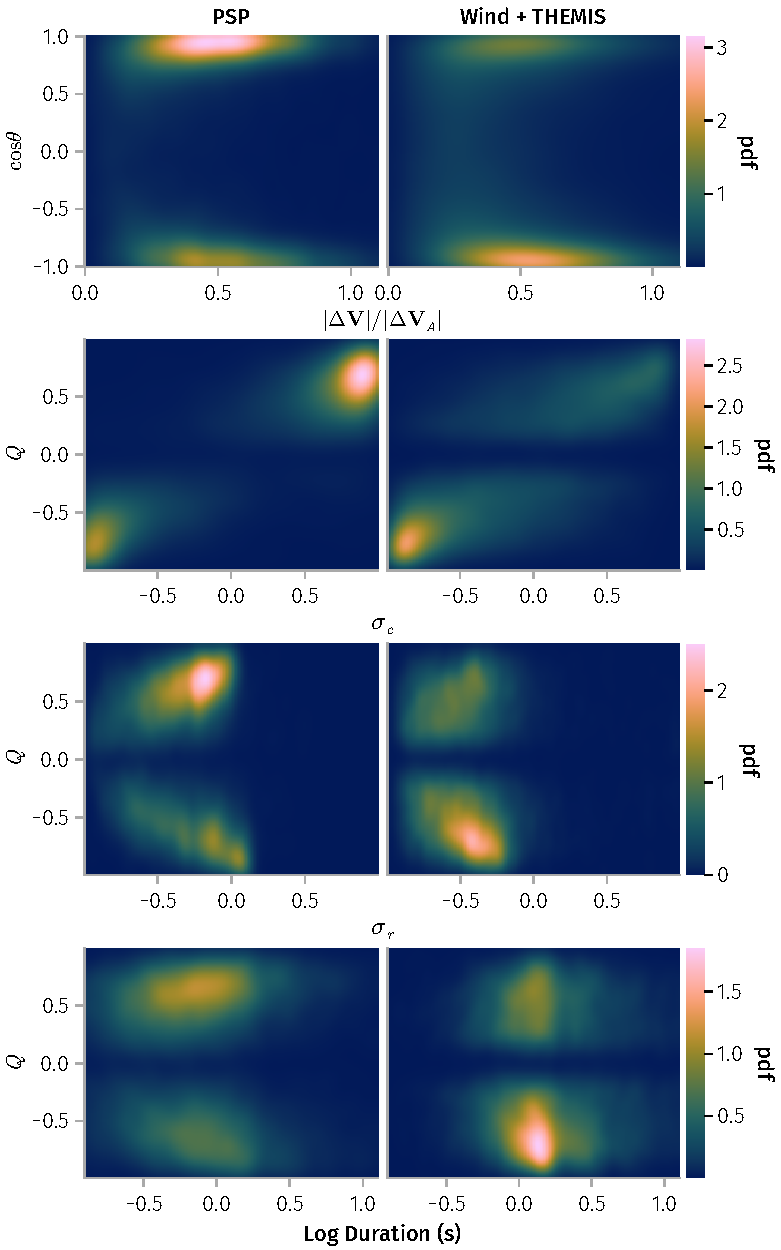
\includegraphics[keepaspectratio]{figures/Q_sonnerup_joint_dist_den.png}}

\begin{enumerate}
\def\labelenumi{(\alph{enumi})}
\tightlist
\item
  Joint distribution of the velocity-jump ratio (\(|\Delta 𝐕| / |\Delta 𝐕_A|\)) and the cosine of the alignment angle (\(\cos \theta\)), used in computing the Sonnerup (\(Q^{\pm}\)) parameter. (b) Joint distribution of cross helicity (\(\sigma_c\)) and (\(Q^{\pm}\)). (c) Joint distribution of residual energy (\(\sigma_r\)) and (\(Q^{\pm}\)). (d) Joint distribution of temporal duration and (\(Q^{\pm}\)).
\end{enumerate}

}

\caption{\label{fig-Q_sonnerup_joint_dist_den}}

\end{figure}%

We examine the relationship between \(Q^{\pm}\) and various current sheet and ambient solar wind properties. Most parameters show little or no correlation with \(Q^{\pm}\); however, two quantities exhibit strong correlations: the cross helicity \(\sigma_c\) and residual energy \(\sigma_r\) of the surrounding solar wind. These parameters describe, respectively, the degree of velocity--magnetic field correlation and the partition of energy between velocity and magnetic field fluctuations. Both serve as indicators of the Alfvénic character of the background solar wind rather than of individual current sheets.

Panels (b) and (c) of Figure~\ref{fig-Q_sonnerup_joint_dist_den} show that the Alfvénicity of current sheets, represented by \(Q^{+}\), increases with higher cross helicity and larger (more positive) residual energy, while \(Q^{-}\) increases with higher cross helicity and smaller (more negative) residual energy. This trend suggests that current sheets embedded within highly Alfvénic solar wind streams tend to preserve stronger velocity--magnetic field alignment, whereas those located in more turbulent or energy-imbalanced regions---where magnetic energy \((E_B)\) exceeds kinetic energy \((E_V)\)---exhibit greater departures from Alfvénic expectations.

Additionally, observations reveal a weak positive correlation between \(Q^{\pm}\) and the temporal duration of current sheets, as shown in Panel (d) of Figure~\ref{fig-Q_sonnerup_joint_dist_den}. Longer-duration current sheets tend to exhibit slightly higher \(Q^{\pm}\) values, suggesting a more coherent Alfvénic structure. However, this correlation may be partially influenced by instrumental limitations, since longer events are more reliably resolved in plasma velocity measurements. Other plasma parameters, such as plasma beta and alpha-particle abundance, show no significant correlation with \(Q^{\pm}\), implying that the Alfvénic nature of current sheets is primarily governed by the local turbulent environment rather than by large-scale plasma conditions.

Since the normal component of the magnetic field plays a key role in determining both the spatial scale and the associated current density, we next examine the rotational characteristics of the current sheets and their relationship with the normalized normal magnetic field component, \(B_N/B\).
Figure~\ref{fig-B_n_ω} shows the distributions of the in-plane rotation angle (also referred to as the shear angle) and the normalized normal component \(B_N/B\), along with their joint distributions for different missions. Panel (a) reveals that PSP observes a distinctly different distribution of rotation angles compared to the Wind and ARTEMIS missions, while the distributions of \(B_N/B\) are largely similar, as shown in Panel (b). This discrepancy suggests that the rotational structure of current sheets evolves significantly as the solar wind propagates from the near-Sun environment to 1 AU.
The multiple peaks in PSP's in-plane rotation angle distribution likely reflect the coexistence of several current sheet populations, possibly formed through different mechanisms or originating from different solar wind sources. As the solar wind expands and mixes, this structured distribution becomes smoother, as observed by Wind and ARTEMIS near Earth.
The distribution of \(B_N / B\) is clearly bimodal, with one population corresponding to nearly field-aligned normals and another to nearly perpendicular ones. Only a small fraction of events fall in the intermediate range. Such bimodal distributions are consistent with the coexistence of different types of discontinuities---most notably rotational and tangential discontinuities \citep{madarDirectionalDiscontinuitiesInner2024}.
Panel (c) shows the joint distribution of the in-plane rotation angle and \(B_N / B\), where each column has been normalized to highlight how the rotation angle varies with \(B_N / B\). The distinct distribution observed by PSP again indicates an evolutionary trend: current sheets closer to the Sun exhibit a more structured and varied rotational behavior, which gradually transitions to smoother and more uniform configurations at 1 AU.

\begin{figure}

\centering{

\pandocbounded{\includegraphics[keepaspectratio]{figures/B_n_ω_-mva-subset=true.png}}

\begin{enumerate}
\def\labelenumi{(\alph{enumi})}
\tightlist
\item
  Probability density functions of the in-plane rotation angle (\(\omega_{\text{in}}\)) for Parker Solar Probe (PSP) and Wind + THEMIS. (b) Probability density functions of the normalized normal magnetic field component (\(B_N / B\)). (c) Joint distributions of \(\omega_{\text{in}}\) and \(B_N / B\) for PSP (left) and Wind + THEMIS (right).
\end{enumerate}

}

\caption{\label{fig-B_n_ω}}

\end{figure}%

Finally, Figure~\ref{fig-duration} presents the probability density functions of current sheet temporal durations observed by different missions. The distributions differ noticeably in shape, reflecting variations in the relative occurrence of short- and long-duration events among the datasets. The gradual change in slope with increasing duration suggests the presence of at least two, and possibly three, distinct regimes contributing to the overall range of current sheet durations.
The shortest-duration events are likely associated with kinetic-scale current sheets, while the longer-duration events may correspond to flux-tube boundaries, large-scale magnetic structures, or heliospheric current sheets. The similar slopes observed at longer durations across missions indicate that large-scale structures are relatively stable with heliocentric distance, whereas the short-duration population evolves more rapidly as the solar wind expands.
Assuming that current sheets propagate radially without significant distortion or dissipation, the measured temporal duration can be interpreted as a proxy for the spatial thickness of the structure, modulated by the magnetic field orientation. To account for geometric effects, we apply a correction based on the Parker spiral model, multiplying the PSP durations by the factor \(\sin(\Theta_{\text{Earth}}) / \sin(\Theta_{\text{PSP}})\), where \(\Theta \approx \arctan(B_T / B_R)\) is the angle between the magnetic field and the radial direction, with \(B_R\) and \(B_T\) denoting the radial and transverse magnetic field components, respectively. Although this correction is a simplified approximation and not physically rigorous, it provides a useful scaling comparison: after adjustment, the PSP duration distribution aligns closely with those of Wind and ARTEMIS near 1 AU for short-duration current sheets. This agreement suggests that the shortest-duration (kinetic-scale) current sheets are predominantly oriented perpendicular to the mean magnetic field and evolve substantially with distance from the Sun.

\begin{figure}

\centering{

\pandocbounded{\includegraphics[keepaspectratio]{figures/duration_dist.png}}

}

\caption{\label{fig-duration}Probability density functions of current sheet durations observed by different missions. Grey vertical dashed lines indicate durations of 1, 2, 4, 8, 16, and 32 s (from left to right).}

\end{figure}%

\section{Conclusion}\label{conclusion}

\begin{enumerate}
\def\labelenumi{\arabic{enumi}.}
\item
  We investigated three Parker Solar Probe (PSP) encounters, complemented by ARTEMIS and Wind measurements, to identify and characterize current sheets across different heliocentric distances. The results indicate that variations in the selected time intervals exert only a minor influence on key current sheet properties such as thickness, current density, and Alfvénicity. This suggests that the observed evolution of current sheet characteristics primarily reflects spatial effects associated with radial expansion rather than temporal variability.
\item
  Our analysis confirms that current sheet properties are closely linked to local plasma conditions and extends previously reported scale-dependent relationships between current sheet thickness and current density by more than two orders of magnitude, encompassing structures from kinetic to large MHD scales. Both the normalized current density and normalized thickness remain nearly constant across radial distances, with only a slight decrease in normalized thickness farther from the Sun. The pronounced anti-correlation between current density and spatial scale---stronger current densities corresponding to thinner sheets---and the similarity of normalized current densities across radial distances indicate a close connection between current sheets and MHD turbulence, since localized, non-Gaussian current density enhancements are a hallmark of intermittency in turbulent plasmas.
\item
  The Alfvénicity of most current sheets, quantified by the parameter \(Q\), remains below unity for the majority of events. The magnitude ratios reported by PSP and Wind are broadly consistent, while PSP observations show smaller angular deviations than those from Wind and ARTEMIS. Pressure anisotropy alone does not account for the observed velocity and magnetic field jumps. Instead, the degree of Alfvénicity appears to be primarily controlled by the surrounding turbulent plasma state---specifically, by cross helicity and residual energy. Most current sheets are nearly force-free, exhibiting low compressibility (typically \textless0.1). These findings support a picture in which current sheets are embedded within, and shaped by, the local turbulent cascade rather than being isolated structures produced by single local processes. In other words, the macroscopic turbulence environment determines whether a boundary appears Alfvénic or non-Alfvénic when sampled in situ.
\end{enumerate}

\begin{enumerate}
\def\labelenumi{\arabic{enumi}.}
\setcounter{enumi}{3}
\tightlist
\item
  A comparison between PSP and near-Earth missions reveals that the statistical properties of solar wind current sheets undergo systematic evolution with heliocentric distance. Clear differences are observed in the distributions of unnormalized current density, thickness, magnetic field jump, rotation angle, and temporal duration. Processes that may drive this evolution include global solar wind expansion \citep{matteiniIonKineticsSolar2012}, nonlinear dynamics of Alfvén waves and Alfvénic turbulence \citep{medvedevDissipativeDynamicsCollisionless1997}, and interactions with other coherent structures. This evolution has important implications for the role of current sheets in plasma heating \citep{sioulasStatisticalAnalysisIntermittency2022}, particle energization and transport \citep{zhangQuantificationIonScattering2025}, which are expected to depend strongly on radial distance.
\end{enumerate}

Taken together, our results support a picture in which current sheets are predominantly turbulence-embedded, dynamically evolving structures whose Alfvénic character is governed by the ambient solar wind turbulence---through cross helicity and residual energy. The tight coupling between current sheet intensity and spatial scale, the coexistence of at least two structural regimes, and the systematic radial evolution of their properties collectively point to a complex interplay between turbulent intermittency, solar wind expansion, and kinetic processes. Resolving these remaining discrepancies will require higher-resolution particle measurements, multi-spacecraft observations, and dedicated kinetic modeling.

\section{Appendix}\label{appendix}

\begin{figure}

\centering{

\pandocbounded{\includegraphics[keepaspectratio]{figures/properties_hist-cross.png}}

}

\caption{\label{fig-properties-hist-cross}Same as Figure~\ref{fig-properties-hist} but using cross product to determine the normal direction to the current sheet.}

\end{figure}%

\begin{figure}

\centering{

\pandocbounded{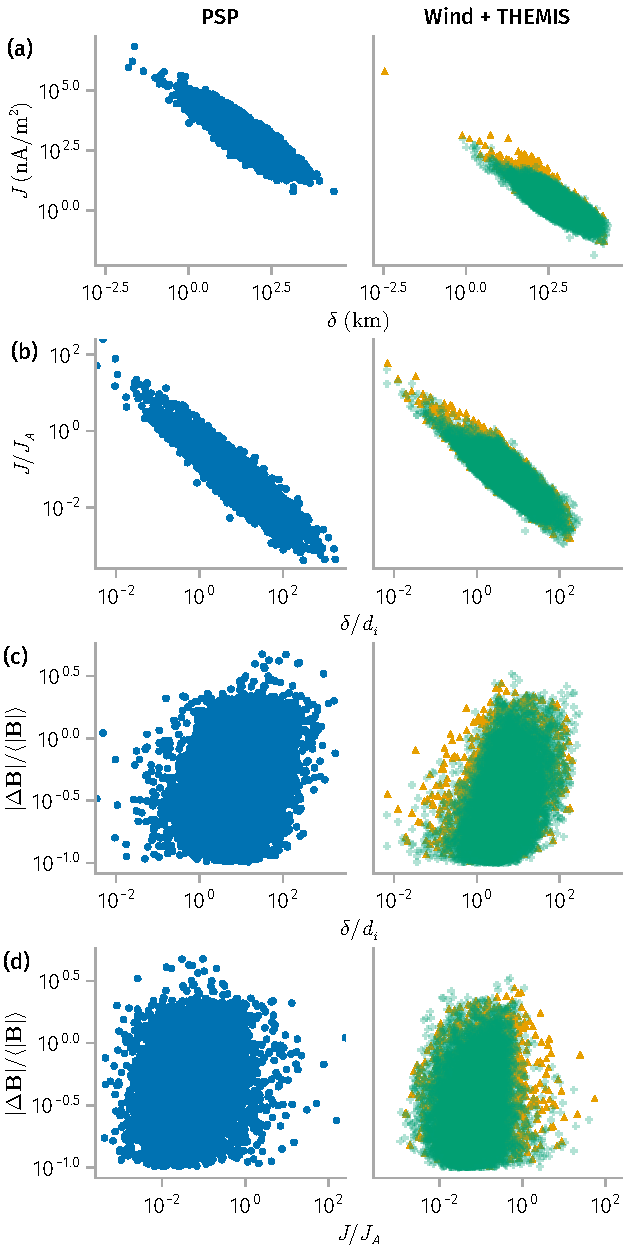
\includegraphics[keepaspectratio]{figures/joint_properties-cross.png}}

}

\caption{\label{fig-joint-properties-cross}Same as Figure~\ref{fig-joint-properties} but with current sheet normals determined using the magnetic field cross-product method instead of minimum variance analysis (MVA).}

\end{figure}%


\bibliography{files/bibliography/research.bib}



\end{document}
